
\documentclass[11pt]{article}

\usepackage[margin=1in]{geometry}
\usepackage{graphicx}
\usepackage{amsmath, amssymb, amsthm}
\usepackage{booktabs}
\usepackage{array}
\usepackage{hyperref}
\usepackage{enumitem}
\usepackage[T1]{fontenc}
\usepackage{lmodern}
\usepackage{float}

\title{CPSC 448 Directed Studies Final Report\\Systematic Testing of Concurrency Schedules in Go-based Distributed Systems}
\author{Allan Tan}
\date{Winter 2025 Term 2\\Supervisors: Arpan Gujarati, Ivan Beschastnikh}

\begin{document}

\maketitle

\section{Introduction}

Testing distributed systems is a complex challenge. The difficulty of testing stems from non-deterministic concurrency and the presence of ``Heisenbugs'' -- bugs that occur but disappear or change when you observe them. Currently, stress testing is used to identify breaking points and simulate real load, but it often fails to replicate specific interleavings that are error prone and could cause critical failures in production. While tools like Go's experimental Synctest package assist with concurrency testing within a single program, there is no existing out-of-the-box solution for testing goroutine interleavings between multiple, communicating Go programs. This is a significant gap in testing distributed systems as concurrency bugs arise from complex inter-service dependencies.


This research proposes a testing framework ``Bubbles,'' that has been extended from Synctest. Bubbles systematically tests the cross product of interleavings between global messages between nodes and local goroutines by isolating nodes, controlling schedulable operations, and deploying specific scheduling algorithms to reduce the search space and find bugs. Bubbles can be used as a local testing tool similar to Go's race detector, or it can be used to find bugs in a distributed system. This final report focuses on how Bubbles works at the global level and benchmarks it against a couple simple example distributed systems.

\section{Overview}

\subsection{Bubbles and the System Model}

The orchestrator has two main responsibilities: deterministically scheduling operations between bubbles, and exploring multiple interleavings until the test passes or a bug is found. Each bubble is an isolated execution environment with its own fake clock, a closed set of goroutines, and a communication mechanism that sends the state of the bubble to the orchestrator when a yield point is hit.

At each yield point, the bubble exposes its state to the orchestrator, which contains a runnable set $R = \{g_1, g_2, \ldots, g_n\}$ --- the set of goroutine IDs eligible to run next. Scheduling decisions occur when the program yields to different goroutines. This is where execution can take a different path depending on a non-deterministic choice. Yield points include channel sends, channel receives, \texttt{select}, locks, wait groups, goroutine exits, or explicit goroutine scheduling.

At the orchestrator level, nodes in a distributed system map to one synctest bubble and each bubble is mapped to one logical processor ($P$) that has mid-execution preemption disabled. A single $P$ ensures that at most one goroutine in the bubble can run at a time, making every scheduling choice sequential and observable. A three-node cluster becomes three bubbles, each running its own goroutines in isolation. Each node's requests to other nodes are proxied through the orchestrator where it can be observed and controlled. When all nodes in the system are blocked from making progress, the orchestrator will decide which schedulable operation to run from a queue. This serializes the operations that run in a test and produces a trace that enables deterministic replay in the case that a bug is found.

With all the local and global operations available to the orchestrator, it can explore interleavings at both levels. At the global level, the orchestrator varies the order in which cross-node messages are delivered across runs. At the local level, it varies which goroutine within a node runs next at each yield point. These scheduling decisions are chosen using a configured scheduling algorithm that systematically or probabilistically explores the search space. A single test execution fixes one choice at each of these decision points; exploring interleavings means re-running the system with different choices and checking whether any combination triggers a bug.

\subsection{Schedulable Operations, Decision Points, and the Trace}

At any given moment during a distributed test, there are two kinds of choices the framework must make: which goroutine to run next inside a node, and which cross-node message to deliver next. These are called \emph{local} and \emph{global} schedulable operations respectively.

Local operations are the goroutines in the runnable set R of a single bubble. When a bubble has multiple runnable goroutines the scheduler must pick one. In normal Go execution, this choice is made pseudo-randomly. In Bubbles, it becomes a controlled decision point that can be exploited to find hidden bugs. Global operations are pending messages that have been sent but not yet delivered. When node A sends a message to node B, it is withheld until the orchestrator chooses to deliver it. All pending operations across all nodes accumulate in a global queue, and the orchestrator executes one operation when all nodes are idle. 

The orchestrator records all decision points made during a single execution and flattens them into a unified trace
\[
\mathcal{U} = \langle s_1, s_2, \ldots, s_m \rangle,
\]
an ordered sequence of all steps taken. Each step in the trace is a tuple
\[
s = (k, n, i),
\]
where \(k \in \{L, G\}\) denotes the kind (local or global), \(n\) is the number of alternative decisions available at that point, and \(i \in \{0, \ldots, n-1\}\) is the chosen index. The default choice \(i = 0\) corresponds to FIFO order; any step with \(i \neq 0\) is a non-FIFO decision.

The trace serves two purposes. First, it enables exact replay: a prefix
\[
P = \langle s_1, \ldots, s_\ell \rangle, \quad \ell \leq m,
\]
can be fed back to the orchestrator to reproduce the first \(\ell\) choices of that execution. Second, it is the input to the search algorithm: after each run, the algorithm identifies steps with unexplored alternatives (i.e., steps \(s_j\) where \(i_j < n_j - 1\)) and produces new prefixes that branch at those points, driving the next run.


\subsection{The Orchestrator Cycle}

Testing with Bubbles requires the developer to simply wrap their existing tests with the orchestrator APIs and implement the transport layer interface to enable channel based communication. Bubbles expects that most distributed system test suites already have helper functions to spin up nodes, connect them, and configure the cluster, and so the setup is structurally very simple. 

Once set up, exploration proceeds as follows:

\begin{description}[leftmargin=0pt,labelindent=0pt]
\item[\textbf{Step 1 --- Baseline.}] The first run executes entirely in FIFO order, establishing a baseline trace $T = \langle s_1, s_2, \ldots, s_m \rangle$.

\item[\textbf{Step 2 --- Run.}] Each subsequent run is guided by a prefix $P$. The orchestrator executes the distributed system serially --- one operation at a time across all nodes:
\begin{itemize}[leftmargin=1.5em]
    \item \textbf{2a --- Wait.} The orchestrator waits until every active node is \emph{idle} --- all goroutines inside every bubble are durably-blocked and cannot make further progress. As each node goes idle it drains its outbox into the global queue $Q$.
    \item \textbf{2b --- Transition.} Once all active nodes are idle, the orchestrator picks a transition in priority order:
    \begin{itemize}[leftmargin=1.5em]
        \item \textbf{Deliver}: If $Q \neq \emptyset$, pick one operation using either the prefix $P$ (if steps remain) or the configured scheduling algorithm (at the frontier). Deliver it to its target node and await that node's next idle report.
        \item \textbf{Advance}: If $Q = \emptyset$ and at least one node has a pending timer, advance fake time $\tau$ to the nearest timer and resume the affected nodes.
        \item \textbf{Drain}: If $Q = \emptyset$ and no pending timers exist, delegate idle handling to the synctest runtime (which either advances its own clock or detects deadlock).
    \end{itemize}
    \item \textbf{2c --- Repeat.} Steps 2a--2b repeat until all nodes have finished, producing the complete trace $T$ for this run.
\end{itemize}

\item[\textbf{Step 3 --- Check.}] If any node's assertions fail, a bug has been found. The trace $T$ is the exact sequence of decisions that triggered it and can be replayed deterministically to reproduce the failure.

\item[\textbf{Step 4 --- Branch.}] If no bug was found, the orchestrator identifies steps in $T$ with unexplored alternatives --- steps $s_j$ where $i_j < n_j - 1$. Each such step produces a new prefix: the decisions of $T$ up to step $j$, with the choice at $j$ changed to an unexplored alternative. Prefixes whose non-FIFO count exceeds the bound $k$ are discarded.

\item[\textbf{Step 5 --- Repeat.}] Exploration continues with the newly generated prefixes, cycling through Steps 2--4 until no unexplored alternatives remain within the bound or a bug is found.
\end{description}

\section{Orchestrator Formal Model}

This section formally defines the orchestrator. 

\subsection{Global State}

At any point during a run the orchestrator is described by the tuple
\[
S = (\tau,\; \Sigma,\; Q,\; P,\; \mathcal{U})
\]

\begin{center}
\begin{tabular}{@{}lll@{}}
\toprule
Symbol & Type & Meaning \\
\midrule
$\tau$ & $\mathbb{Z}_{\geq 0}$ & Current global fake time (nanoseconds) \\
$\Sigma$ & $N \to \{\texttt{running},\, \texttt{idle},\, \texttt{done}\}$ & Per-node execution status \\
$Q$ & $\text{PendingOp}^*$ & Ordered list of schedulable cross-node operations \\
$PM$ & $N \rightharpoonup \text{IdleState}$ & Partial map from idle nodes to their reported idle state \\
$\mathcal{U}$ & $\text{NewStep}^*$ & Unified trace: all recorded decisions (local and global) \\
\bottomrule
\end{tabular}
\end{center}

$N = (n_1, \ldots, n_k)$ is the sequence of nodes that are added to the orchestrator in order. \textbf{Active nodes} $A = \{n_i \in N \mid \Sigma(n_i) \neq \texttt{done}\}$. The orchestrator is \textbf{fully idle} when $\mathrm{dom}(PM) = A$, i.e., every active node has reported to the orchestrator that it's idle.

\subsection{Idle Condition}

A goroutine $g$ inside bubble $B_i$ is \textbf{durably-blocked} if it hit a yield point. The bubble is \textbf{idle} when all of its goroutines are durably-blocked:
\[
\text{Idle}(B_i) \iff \forall\, g \in G(B_i) : \text{durablyBlocked}(g)
\]

When $\text{Idle}(B_i)$ first becomes true, the synctest runtime fires a hook that transmits an \texttt{IdleState} to the orchestrator and blocks until a \texttt{Resume} is sent back to the bubble. This hook is the boundary between the orchestrator's main loop and each bubble's execution.

\subsection{Bubble--Orchestrator Interface}

Each bubble communicates with the orchestrator through a pair of synchronous messages over a per-bubble channel pair:

\begin{description}[leftmargin=0pt,labelindent=0pt]
\item[\texttt{IdleState}] Reported by a bubble the moment $\text{Idle}(B_i)$ first becomes true. It carries the information the orchestrator needs to choose its next transition: the bubble's pending outbox messages and the timestamp of its nearest pending timer (if any).

\item[\texttt{Resume}] Sent by the orchestrator to unblock a waiting bubble. It tells the bubble what to do next: deliver a pending message, advance fake time to a given timestamp (\texttt{AdvanceTimeTo}), or hand idle handling back to the synctest runtime (\texttt{DelegateIdle}).

\item[Hook] The synctest runtime mechanism that detects $\text{Idle}(B_i)$, serializes the \texttt{IdleState}, and suspends the bubble's goroutine until a \texttt{Resume} arrives. The hook runs on the bubble's $P$, so the bubble holds no OS thread while waiting.
\end{description}

\subsection{Main Loop Transitions}

Once the orchestrator is fully idle ($\mathrm{dom}(P) = A$), it chooses one of three transitions in priority order:

\paragraph{Deliver}
If $Q \neq \emptyset$ (after draining all outboxes), the algorithm selects an operation
\[
p = (\text{from}, \text{to}, \text{type}, \text{exec})
\]
from $Q$. Then:
\begin{enumerate}[leftmargin=1.5em]
    \item Remove $p$ from $Q$.
    \item Execute $p$ and deliver it to the target bubble.
    \item Record $\text{Deliver}(p.\text{from}, p.\text{to}, p.\text{type}, \tau)$ in the trace.
    \item Send \texttt{Resume} to $B_{p.\text{to}}$; await its next \texttt{IdleState} or completion.
\end{enumerate}

\paragraph{Advance}
If $Q = \emptyset$ and at least one node has a pending timer:
\[
\tau' = \min_{\substack{n_i \in A \\ \text{nextTimer}(P[n_i]) > 0}} \text{nextTimer}(P[n_i])
\]

Set $\tau \leftarrow \tau'$. Then, in registration order, send \texttt{Resume\{AdvanceTimeTo: $\tau'$\}} to each idle bubble and await its next event.

\paragraph{Drain}
If $Q = \emptyset$ and no node has a pending timer, the system has no work and no timers --- goroutines are waiting for external input that will never arrive through the message queue. Send \texttt{Resume\{DelegateIdle: true\}} to each idle bubble in registration order, delegating idle handling to the synctest runtime so it can advance its own clock or detect deadlock.

\subsection{Invariants}

The following invariants hold throughout every orchestrator run:

\begin{description}[leftmargin=0pt,labelindent=0pt]
    \item[\textbf{I1 --- At most one active bubble.}] At any point in the delivery or time-advance phase, at most one bubble has $\Sigma(n_i) = \texttt{running}$. Local decisions (which goroutine runs next within a bubble) fire synchronously inside the hook while the orchestrator goroutine is blocked.
    \item[\textbf{I2 --- Sequential rand access.}] No two goroutines from distinct bubbles call randomness functions concurrently.
    \item[\textbf{I3 --- Message causality.}] A message $p$ is only delivered after the sender's bubble has gone idle with $p$ in its outbox. No message can be observed by a receiver before the sender has sent it.
    \item[\textbf{I4 --- Monotone clock.}] $\tau$ is non-decreasing. Each \texttt{Resume\{AdvanceTimeTo: $\tau'$\}} satisfies $\tau' \geq \tau$.
    \item[\textbf{I5 --- No concurrent operations.}] The orchestrator only schedules one operation at a time, so no two bubbles can run at the same time.
    \item[\textbf{I6 --- Algorithm controls all decisions.}] Every scheduling choice --- both local (goroutine order within a bubble) and global (message delivery order across bubbles) --- flows through the scheduling algorithm. This is the single point of control for systematic exploration.
\end{description}

These invariants allow the orchestrator to serialize all operations and enable determinism. 

\subsection{Determinism}

For replay and systematic exploration to work, the same prefix must produce the same execution every time. Let $R_1$ and $R_2$ be two runs of the same test with the same algorithm and initial configuration. Their unified traces $\mathcal{U}_1$ and $\mathcal{U}_2$ are equal if and only if all three of the following conditions hold simultaneously:

\begin{enumerate}[leftmargin=1.5em]
    \item \textbf{Local schedule identity.} For every node $n_i$, $\mathcal{A}.\text{Decide}$ returns the same index at every Local decision point. This is guaranteed by \texttt{GOMAXPROCS=1} (a single logical processor so goroutines cannot run in parallel), \texttt{GODEBUG=asyncpreemptoff=1} (no asynchronous preemption so goroutines only yield at explicit blocking points), and the forked runtime routing \texttt{cheaprand()} tie-breaking through the decision hook instead of the PRNG.

    \item \textbf{Global delivery identity.} $\mathcal{A}.\text{Decide}$ returns the same index at every Global decision point, selecting the same message $(\text{from}, \text{to}, \text{type})$ at the same position in $Q$. This is enforced structurally by the orchestrator: only one global decision is made at a time and all alternatives are fully enumerated before any is taken.

    \item \textbf{Application randomness identity.} Any \texttt{math/rand} calls made by application code use the same seed and occur in the same order. This condition is not enforced by the orchestrator --- callers must seed \texttt{math/rand} deterministically (e.g. \texttt{rand.Seed(42)}) in the per-run setup callback.
\end{enumerate}

If any condition fails, $\mathcal{U}_1 \neq \mathcal{U}_2$ in general. Violating (1) changes which goroutine runs at a yield point, altering when and how many messages are produced. Violating (2) changes which message is processed first, changing application state and all subsequent decisions. Violating (3) changes values like election timeouts that influence which code path runs, independently of the scheduling order.

\paragraph{Replay.}
\texttt{Replay(rec)} re-runs the system following only the Global decisions from a recorded run. At each Global decision point the replay function checks that the recorded queue size matches the current $|Q|$ --- if not, it panics with \texttt{replayDivergenceError}, marking the run as diverged and discarding it. Local decisions always return 0 (FIFO) during replay. Replay is sound when all three conditions hold; a divergence indicates that condition (2) has failed, typically because application-level randomness (condition 3) produced a different message ordering.

\paragraph{Prefix replay and divergence pruning.}
CHESS and DPOR replay a \emph{prefix} --- a prefix $P = \langle s_1, \ldots, s_\ell \rangle$ fixes the first $\ell$ decisions and lets the algorithm choose freely afterward. At each replayed step, the algorithm checks that the recorded \texttt{Kind} and \texttt{Node} match the current decision point. A mismatch (e.g. a local decision appeared where a global one was expected) triggers \texttt{replayDivergenceError}, which the orchestrator catches and uses to prune that branch from the search tree rather than reporting a spurious failure.

\section{Search Algorithms}

The search space in a distributed system is extremely large as many possible interleavings exist. At each decision point, there are multiple goroutines or messages to schedule, and a test with $m$ decision points each with $n$ alternatives has up to $n^m$ possible traces. In practice, it will take a long time to exhaustively explore this space. The orchestrator exposes a pluggable algorithm interface so that different strategies can be used to explore this space. All algorithms share the same configurable properties: a non-FIFO bound $k$, a maximum run budget, and an optional mode that restricts branching at the global level, local level, or both. This section will explain at a high level how each algorithm works, and following sections will evaluate each against example systems. 

\subsection{CHESS --- Context-Bounded DFS}

CHESS bounds exploration by a parameter $k$ that limits how many non-FIFO decisions any single trace may contain. At the frontier, once the prefix is exhausted, CHESS always picks index 0 (FIFO). After each run it generates new prefixes by branching at every step with unexplored alternatives, discarding any that would exceed $k$ non-FIFO decisions. This guarantees complete coverage of all interleavings reachable within the bound. This keeps the search space small while still catching most vulnerable bugs, since most concurrency bugs need only 1-2 non-default scheduling choices to trigger [CHESS SOURCE Source].


CHESS can also operate in global-only mode, branching exclusively on message delivery order while leaving local goroutine scheduling at FIFO, or in global+local mode, branching on both dimensions. The global-only mode is cheaper and sufficient when bugs are caused purely by message reordering, whereas the combined mode is needed when local goroutine races also play a role.

\begin{center}
\begin{tabular}{@{}ll@{}}
\toprule
Property & Value \\
\midrule
Complete & Yes --- all interleavings within bound $k$ \\
Termination & Yes --- finite search space for fixed $k$ \\
Deterministic & Yes --- identical results every run \\
\bottomrule
\end{tabular}
\end{center}

The key weakness of CHESS is that $k$ is a hard ceiling on non-FIFO decisions per trace. Bugs that require many accumulated out-of-order decisions are structurally unreachable regardless of how many runs CHESS performs.

\subsection{PCT --- Probabilistic Concurrency Testing}

PCT assigns random priorities to every schedulable entity and introduces $d - 1$ randomly sampled priority change points per run. At each change point, the currently winning entity is demoted below all others to force a different decision. This gives PCT a theoretical lower bound on bug-finding probability of at least $\frac{1}{n \cdot k^{d-1}}$ per run, where $n$ is the number of schedulable entities and $d$ is the depth parameter [INSERT SOURCE].

Entities in Bubbles are anything that can be scheduled. When choosing global entities, we group messages by type - for example "msg:A→B(Request)”. Local entities are individual goroutine IDs such as “B5”. 

The depth parameter $d$ controls how many priority inversions happen per run --- $d=2$ means one flip, $d=3$ means two. A higher $d$ results in finding deeper bugs, but the probability of hitting those bugs is reduced.

\begin{center}
\begin{tabular}{@{}ll@{}}
\toprule
Property & Value \\
\midrule
Complete & No --- probabilistic, not exhaustive \\
Termination & No --- requires max-runs cap \\
Deterministic & Yes per run, if seeded \\
Bug-finding guarantee & $\geq 1/(n \cdot k^{(d-1)})$ per run \\
\bottomrule
\end{tabular}
\end{center}

\subsection{DPOR --- Dynamic Partial-Order Reduction}
DPOR uses dependency relation between scheduling decisions to prune redundant interleavings. Two steps are dependent if reordering them can produce a different observable outcome. DPOR only branches at steps where the chosen alternative is actually dependent on something that happened later in the trace.

Classical DPOR derives its dependency relation from memory accesses where two operations are dependent if they access the same memory location and at least one is a write [INSERT DPOR SOURCE]. This approach requires the program to observe the heap. However, Bubbles does not operate at that level and has no observability into the lower level systems. 

Bubbles takes a new approach and derives its dependency relation to what the orchestrator can observe without runtime memory instrumentation. Global message deliveries conflict when they share a sender or a target node. Local scheduling decisions conflict when they occur within the same node. An alternative step is considered dependent if: (a) the chosen index and the alternative index share a target node, or (b) some later step in the trace is dependent with the alternative. If a later step already “consumes” the alternative choice, the alternative is no longer relevant and the branch is skipped.

This method may over-estimate the dependencies that a system can have and retain branches that are truly independent, but it will never discard branches that truly matter. This turns out to be reasonably fit for distributed systems as conflicts usually arise when the order in which requests to the same node or goroutines in the same node are interleaved. 

\begin{center}
\begin{tabular}{@{}ll@{}}
\toprule
Property & Value \\
\midrule
Complete & No --- explores dependencies, not exhaustive $k$ \\
Termination & No ––– requires max-runs cap \\
Deterministic & Yes --- identical results every run \\
Pruning & Skips independent interleavings \\
\bottomrule
\end{tabular}
\end{center}

\subsection{Random}

At every decision point, Random picks uniformly at random among all alternatives. It serves as a baseline: it finds bugs eventually if the per-run probability is non-negligible, but offers no guarantees on how many runs are needed and has no structural bias toward bug-triggering regions of the search space.

\begin{center}
\begin{tabular}{@{}ll@{}}
\toprule
Property & Value \\
\midrule
Complete & No \\
Termination & No --- requires max-runs cap \\
Deterministic & Yes per run, if seeded \\
Bug-finding guarantee & None --- depends on run budget \\
\bottomrule
\end{tabular}
\end{center}

\section{Design Choices}


\subsection{Single Runtime}

All nodes run inside a single Go runtime rather than as separate processes. Each node is isolated as a synctest bubble mapped to its own logical processor ($P$), with preemption disabled (\texttt{GOMAXPROCS=1}, \texttt{asyncpreemptoff=1}) so that at most one goroutine runs at a time across the entire system. This design has two main consequences.

\paragraph{What it enables.} The orchestrator intercepts all scheduling decisions via synchronous hooks with no IPC, serialization, or network overhead. Cross-node messages are ordinary Go function calls routed through the transport layer that uses channels.

\paragraph{What it sacrifices.} Bubbles share the same heap. This means that it cannot detect or test real network faults, OS-level scheduling preemption, or serialization bugs that only appear when data crosses a process boundary. It also cannot scale to systems where node count is large enough to exhaust a single process's memory. Although our examples are not large enough to stress this load, this is just a pure limitation of running within a single runtime. 

\subsection{Waiting for Full Idle Before Scheduling}

We decided to preserve Synctest's original durably-blocked semantic as it provided a clear global synchronization boundary where all local computation is blocked. When all bubbles are durably-blocked, it can be viewed as a single ``distributed step'' --- the system has fully reacted to its last input and is waiting for the next one. The orchestrator's job is to choose that next input from $Q$ and advance it to the next state.

If the orchestrator delivered a schedulable operation while some node was still executing, the delivery would race with ongoing local computation. The receiving node's state at the moment of delivery would depend on an arbitrary amount of local progress that had already occurred, making the delivery point neither reproducible nor meaningful as a scheduling decision.

By requiring full idle first, the orchestrator guarantees that the global queue $Q$ is stable. The operations in the queue represent operations that occurred in a single step of the distributed system. Reordering them is meaningful: executing operation $A$ before $B$ versus $B$ before $A$ captures two different executions that could expose a bug. We considered allowing each bubble to run in parallel without full idle, but the downside is that delivering messages mid-run would not produce a clean interleaving. It would produce a different and harder to analyze mixture of local and global non-determinism.

This also gives the execution a clean state-machine structure. Each global step transitions the system from one stable state to the next: all nodes idle $\to$ deliver one message $\to$ run until all nodes idle again. Traces composed of these steps are interpretable, replayable, and comparable across runs, which is what makes systematic exploration tractable.


\subsection{Virtual Clock Advancing}
The orchestrator advances fake time only when the system is fully idle and $Q$ is empty. At that point no pending message can be delivered, so the only possible source of progress is a timer. The orchestrator chooses the minimum pending timer timestamp across all active bubbles, sets $\tau$ to that value, and resumes bubbles with \texttt{AdvanceTimeTo}. This preserves Synctest's fake-clock semantics while making time advancement a deterministic global transition rather than an implicit per-bubble behavior.

We deliberately chose to flush all pending operations before advancing time so that the orchestrator never skips over communication that has already become observable. The cost of that is that time itself is not explored as an independent source of nondeterminism and is not interleaved with other operations. Bubbles does not test clock skew, real time jitter, or interleavings that occur because of timeout races. 

% Transport Layer Interface
\subsection{Transport Layer Interface}

To use Bubbles, the developer implements a thin transport interface that routes all cross-node sends through the orchestrator rather than over a real network. This representation does not lose anything that matters for concurrency testing. The properties of RPCs that produce concurrency bugs are their ordering – which request arrives at a node first, how responses interleave with subsequent requests. Channels preserve these properties and gives explicit control to the orchestrator, whereas network messages would be much harder to intercept. 

% Specific implementation details about the orchestrator


% All bubbles run inside a single Go runtime rather than as separate processes. The primary reason for this is simplicity: synctest’s scheduling hooks are runtime-internal, and wiring them up across process boundaries would require a significant reimplementation. Within a single runtime, the orchestrator intercepts decisions via a hook that fires synchronously with no IPC or serialization overhead.
% This comes with real costs, however. All bubbles share a single heap, so a long-running exploration accumulates allocations across runs and puts pressure on the garbage collector — in practice, GC interactions with the runtime’s bubble state caused crashes during multi-run exploration that required explicit workarounds. There is also no memory isolation between bubbles: a bug in one node’s code can corrupt shared runtime state in ways that affect other nodes, making some failure modes harder to diagnose. A multi-process design would eliminate both problems but would make goroutine-level scheduling interception effectively impossible without cross-process signaling, which would itself introduce non-determinism.


\section{Evaluation}

We evaluated Bubbles' bug finding capabilities by injecting bugs into two simple implementations of distributed systems: (1) a distributed lock bug (ra-gate), (2) a read-repair bug for a replicated key-value store. All experiments ran on a single machine and was repeated for 20 independent seeds. 

\subsection{Distributed Bug: ra-gate}

The ra-gate bug is injected in the Ricart-Agrawala distributed mutual exclusion protocol. Three nodes (A, B, C) share a lock to access a KV store. When a node collects all replies and closes a \texttt{gate} channel, two goroutines wake concurrently: the application goroutine (which sets \texttt{state=Held}) and a deferred-flusher goroutine (which sends deferred replies). Under FIFO local scheduling the application goroutine always runs first. Under non-FIFO scheduling the flusher may observe \texttt{state=Released} and prematurely grant a deferred request, violating mutual exclusion. The full protocol description is in Appendix~\ref{app:ra-gate}.

Finding the bug requires exactly two non-FIFO decisions: (1) a global reordering so a peer's \textsc{Request} arrives while the winner is still collecting replies, causing a deferred reply to queue; and (2) a local reordering that schedules the flusher before the application goroutine after gate close.


\begin{table}[h]
\centering
\caption{ra-gate benchmark results (20 attempts). All algorithms other than CHESS global only find the bug as they explore global + local interleavings, but differ in how many non-FIFO decisions their bug-finding traces contain. CHESS global-only cannot find the bug regardless of run budget.}
\label{tab:ra-gate}

\resizebox{\textwidth}{!}{%
\begin{tabular}{@{}lcccc@{}}
\toprule
Algorithm & Found & Avg runs to bug & Avg non-FIFO in bug run & Avg Total Decisions \\
\midrule
PCT ($d=2$)               & 20/20 & 1.0  & 22.0 & 35.0 \\
Random                    & 20/20 & 2.0  & 13.3 & 35.0 \\
PCT ($d=3$)               & 20/20 & 10.0 & 20.0 & 34.9 \\
DPOR                      & 20/20 & 13.1 & 24.9 & 34.7 \\
CHESS G + L ($k=2$)       & 20/20 & 27.0 & 2.0  & 34.4 \\
CHESS global-only ($k=2$) & 0/20  & ---  & ---  & --- \\
\bottomrule
\end{tabular}%
}
\end{table}

All G+L algorithms find the bug. The algorithms that do not systematically explore (PCT, Random, and DPOR) stumble onto it faster in run count (1--13 runs) but require many non-FIFO decisions. CHESS G+L takes 27 runs but finds the bug with exactly 2 non-FIFO decisions which is the theoretical minimum. CHESS is better suited for finding more shallow bug as it can find the nearest bug-triggering deviation and produce a minimal set of decisions that reproduces the bug. 

CHESS global-only never finds the bug, and that was the expected behavior of this example. Even though this bug is relatively shallow, global only mode never touches the goroutine scheduling, so no matter how large $k$ is or how large our run budget is, it cannot reach the state where DeferredFlusher runs before the App goroutine.

This result highlights a core design decision of the orchestrator: interesting distributed concurrency bugs often arise from the interaction between message ordering and local goroutine scheduling within a node. A framework that controls only message delivery is blind to any bug that requires both dimensions simultaneously.

We constructed a second example to evaluate how the different algorithms behave when the bug is deeper. 

\subsection{Distributed Bug: Quorum Read-Repair}

The quorum-read-repair bug is a data-loss bug in a simplified Dynamo-style replicated key-value store with three replicas (R1, R2, R3). When a reader performs a quorum read and issues read-repair to stale replicas, a sibling value can be lost if the read-repair message is processed by the router goroutine before a concurrent late write has been committed by the apply loop. The bug manifests as a missing sibling in the final quorum read, violating the vector-clock merge semantics. A full description of the system and the bug mechanism appears in Appendix~\ref{app:quorum-read-repair}.

Unlike ra-gate, this bug requires many accumulated non-FIFO decisions spread across a long trace. The router must process the late Put and the Repair consecutively before the apply loop drains, which requires coordinated global delivery ordering and a specific local goroutine sequence inside R1's pipeline.

\begin{table}[h]
\centering
\caption{Quorum-read-repair benchmark results (20 attempts, 2000-run budget). CHESS cannot reach the bug regardless of run budget --- the required non-FIFO depth far exceeds $k=2$. DPOR finds it on every attempt with near-zero variance. PCT is fastest on average but has tail risk.}
\label{tab:qrr}
\begin{tabular}{@{}lcccc@{}}
\toprule
Algorithm & Found & Avg runs to bug & Avg non-FIFO in bug run & Avg total decisions \\
\midrule
DPOR                  & 20/20 & 11.0 & 32.6  & 39.1  \\
PCT ($d=2$)           & 20/20 & 6.6  & 25   & 38.6  \\
PCT ($d=3$)           & 20/20 & 6.6  & 25.1   & 38.6  \\
Random                & 19/20 & 76.5 & 25.9  & 42.6  \\
CHESS G+L ($k=2$)     & 0/20  & ---  & --- & --- \\
CHESS global-only ($k=2$) & 0/20 & --- & --- & --- \\
\bottomrule
\end{tabular}
\end{table}

\begin{figure}[h]
  \centering
  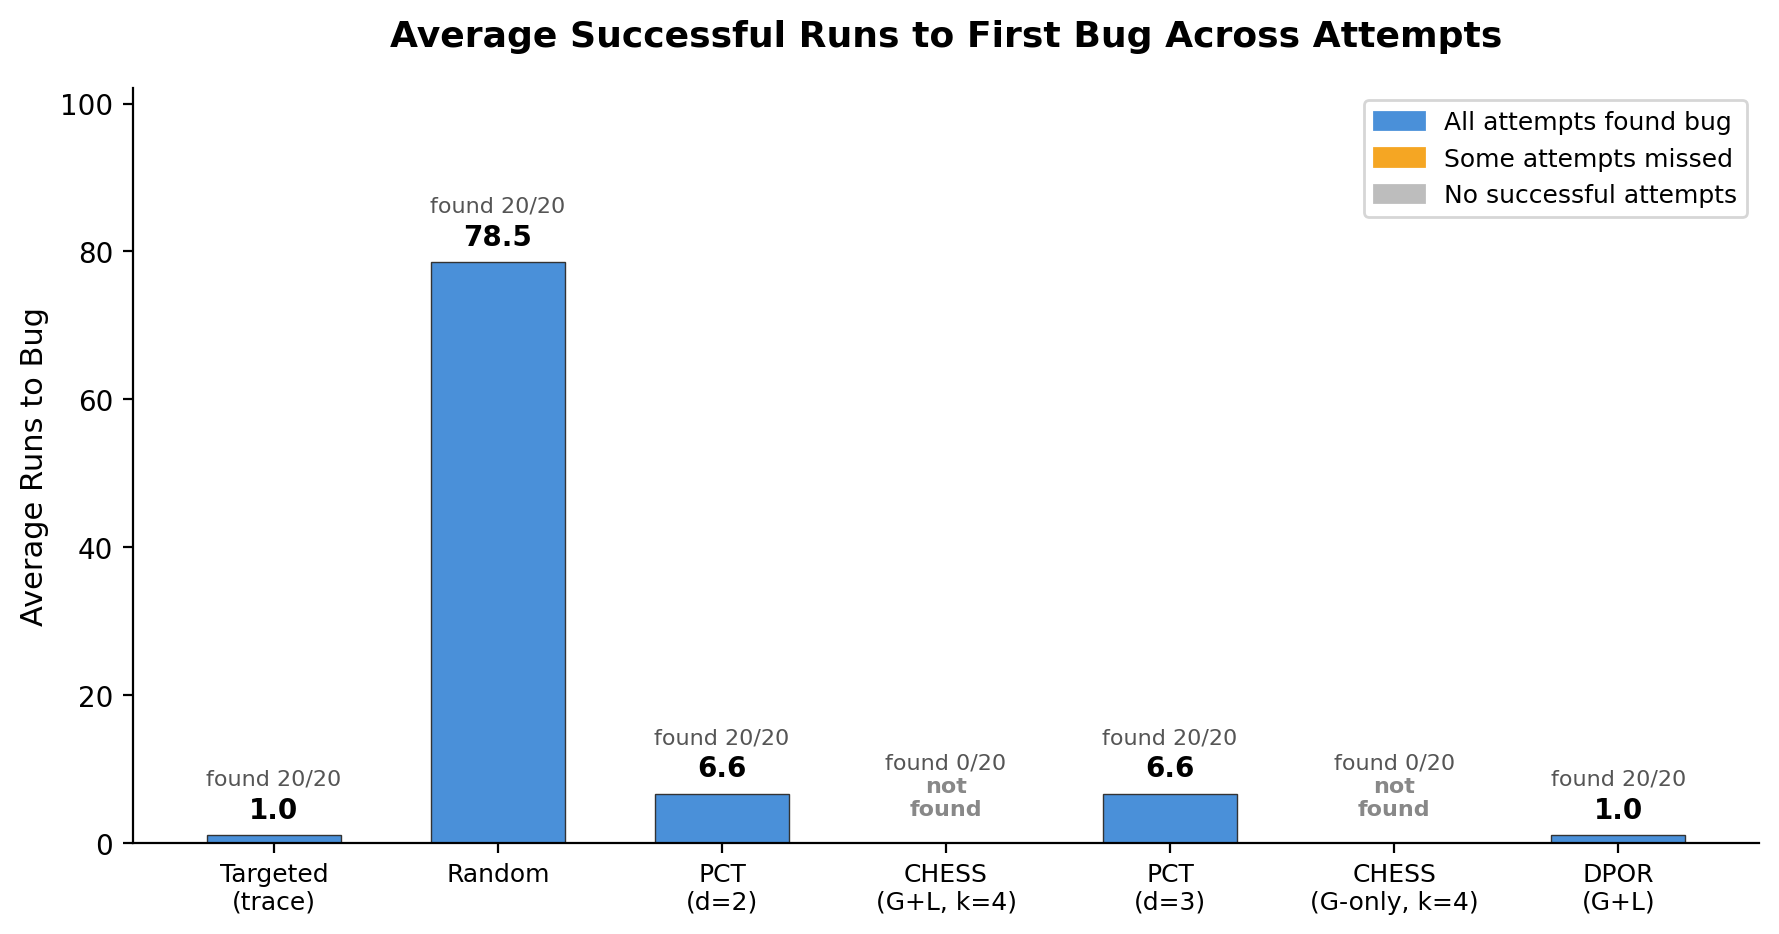
\includegraphics[width=0.72\linewidth]{../../bugs/quorum-read-repair/benchmarking/figures/runs_to_bug.png}
  \caption{Runs to first bug for quorum-read-repair across 20 seeds. CHESS (both variants) never appears --- it finds nothing in 2000 runs. DPOR finds the bug in exactly 11 runs in every attempt. PCT finds it in under 7 runs on average but with a worst case of 26. Random requires ~78 runs on average and one seed fails entirely.}
  \label{fig:qrr-runs}
\end{figure}

We attempted to run Bubbles using CHESS to find this bug using $k$ values 2, 4, 8, 16, 32, 64, 128, 256 with an extremely high run cap, but was not able to find the bug in all attempts. From the other algorithms, the bug is found after ~25 non-FIFO decisions. Even with $k$ = 256, the algorithm only reaches around ~20 non-FIFO decisions. This example demonstrates that systematic DFS exploration isn't fit for all bugs and that adopting other strategies will allow for a more exhaustive exploration.

\begin{figure}[h]
  \centering
  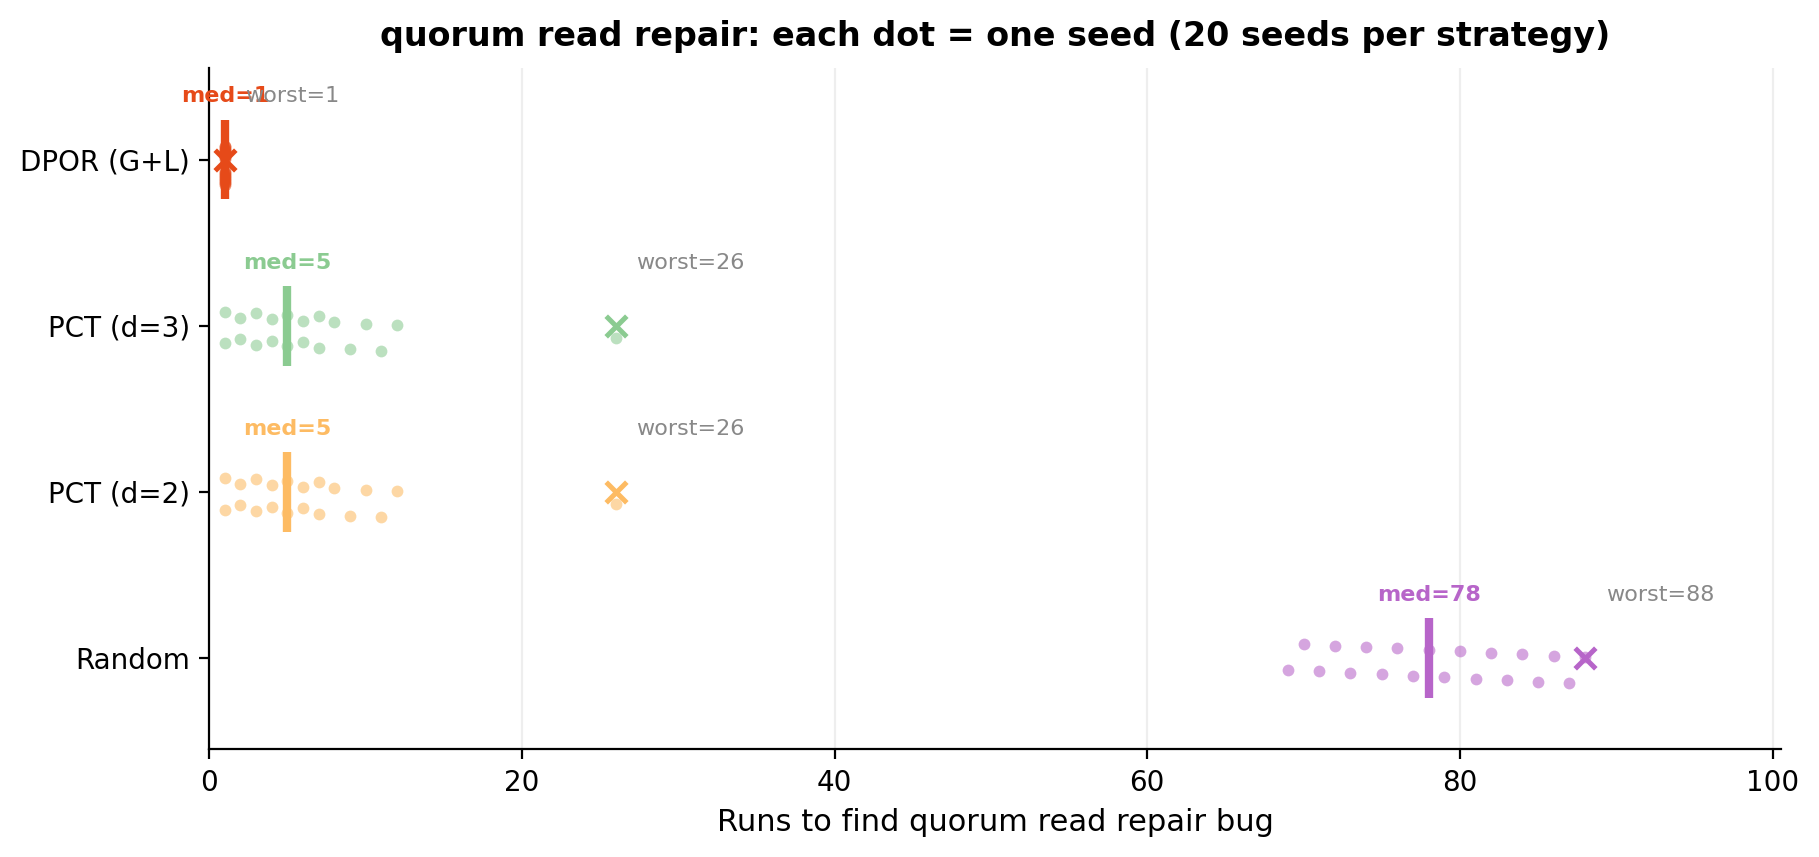
\includegraphics[width=0.72\linewidth]{../../bugs/quorum-read-repair/benchmarking/figures/seed_runs_to_bug.png}
  \caption{Per-seed runs to bug for quorum-read-repair. DPOR's dots form a tight vertical cluster (median 10, worst 11) --- near-zero variance across seeds. PCT shows significant spread (worst case 26). Random's open circle marks the one seed that exhausted the 2000-run budget without finding the bug.}
  \label{fig:qrr-seed}
\end{figure}

DPOR, on the other hand, finds the bug in exactly 11 runs in every single attempt. The reason is that DPOR uses no randomness whatsoever --- its exploration tree is a deterministic mathematical object derived entirely from the program's happens-before structure. A seed is irrelevant to DPOR because DPOR never consults one. Two operations are scheduled as dependent in DPOR if reordering them can change an observable outcome, and the set of dependent pairs is fixed once the program is fixed. From those dependencies, DPOR builds a DFS tree of traces, and the bug-triggering trace occupies a specific node in that tree. Every run of DPOR on this program visits the nodes of that tree in exactly the same order, so the bug is always found at the same position --- in this case, node 11. The 10--11 range of observed variance is not seed variance; it is the result of DPOR's G+L coordination sometimes discovering the critical local race from one global ordering versus a slightly different one, shifting the bug by one DFS step. The contrast with PCT and Random is total: those algorithms find the bug at position $k$ because a random draw landed on the bug-triggering schedule on attempt $k$, so $k$ varies across seeds. DPOR finds the bug at position 11 because that is where node 11 is in the tree, and the tree never changes.

PCT and Random also find the bug, but probabilistically. PCT's median of 5 runs reflects a favorable per-run probability given its priority-inversion mechanism. However, PCT's worst case of 26 runs (over 4$\times$ its median) and Random's single missed seed illustrate the tail risk of probabilistic algorithms. For workloads where a fixed run budget must guarantee bug detection, neither is reliable.

Figure~\ref{fig:qrr-seed} makes the variance structure visible at the per-seed level. DPOR's vertical cluster is the visual signature of determinism: because its exploration tree is fixed, every seed explores the same sequence of traces and reaches the bug at the same position. PCT's wider spread reflects its dependence on random priority assignments --- lucky seeds hit the bug-triggering combination early, unlucky ones take longer. The single open circle for Random represents the one seed where geometric bad luck caused all 2000 runs to miss the required ordering.

\begin{figure}[h]
  \centering
  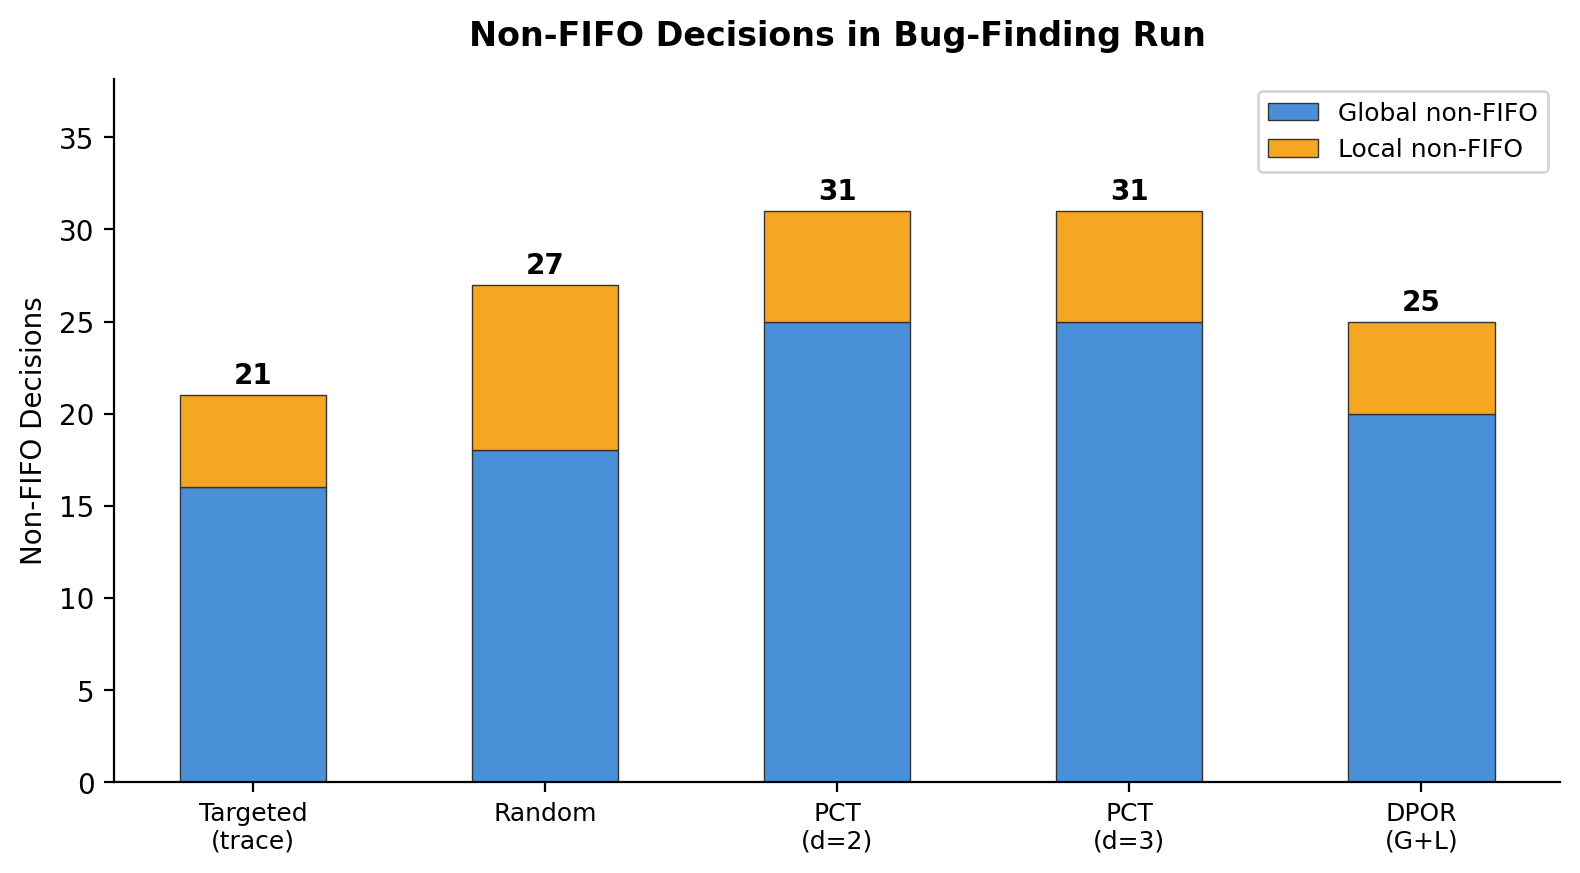
\includegraphics[width=0.85\linewidth]{../../bugs/quorum-read-repair/benchmarking/figures/nonfifo_comparison.png}
  \caption{Non-FIFO decisions in the bug-finding trace for each algorithm. DPOR has the highest total (34), with a notably large local component (15). PCT and Random make fewer non-FIFO decisions overall but take different mixes of global and local inversions.}
  \label{fig:qrr-nonfifo}
\end{figure}

The non-FIFO comparison in Figure~\ref{fig:qrr-nonfifo} reveals a structural difference between DPOR and the probabilistic algorithms. DPOR produces 34 non-FIFO decisions in its bug trace --- more than PCT (31) or Random (27) --- with a particularly large local component of 15. This is not inefficiency; it reflects DPOR's systematic exploration of the local scheduling space. DPOR identifies commutative local goroutine orderings and explores their alternatives explicitly, producing traces with many local inversions as a consequence of thorough coverage. PCT and Random reach the same bug via a single lucky local schedule, touching far fewer local scheduling alternatives along the way. CHESS's $k=2$ ceiling sits at the far left --- a reminder that the minimum observed non-FIFO count in any successful bug-finding trace (27 for Random) is still over 13$\times$ CHESS's bound.

\begin{figure}[h]
  \centering
  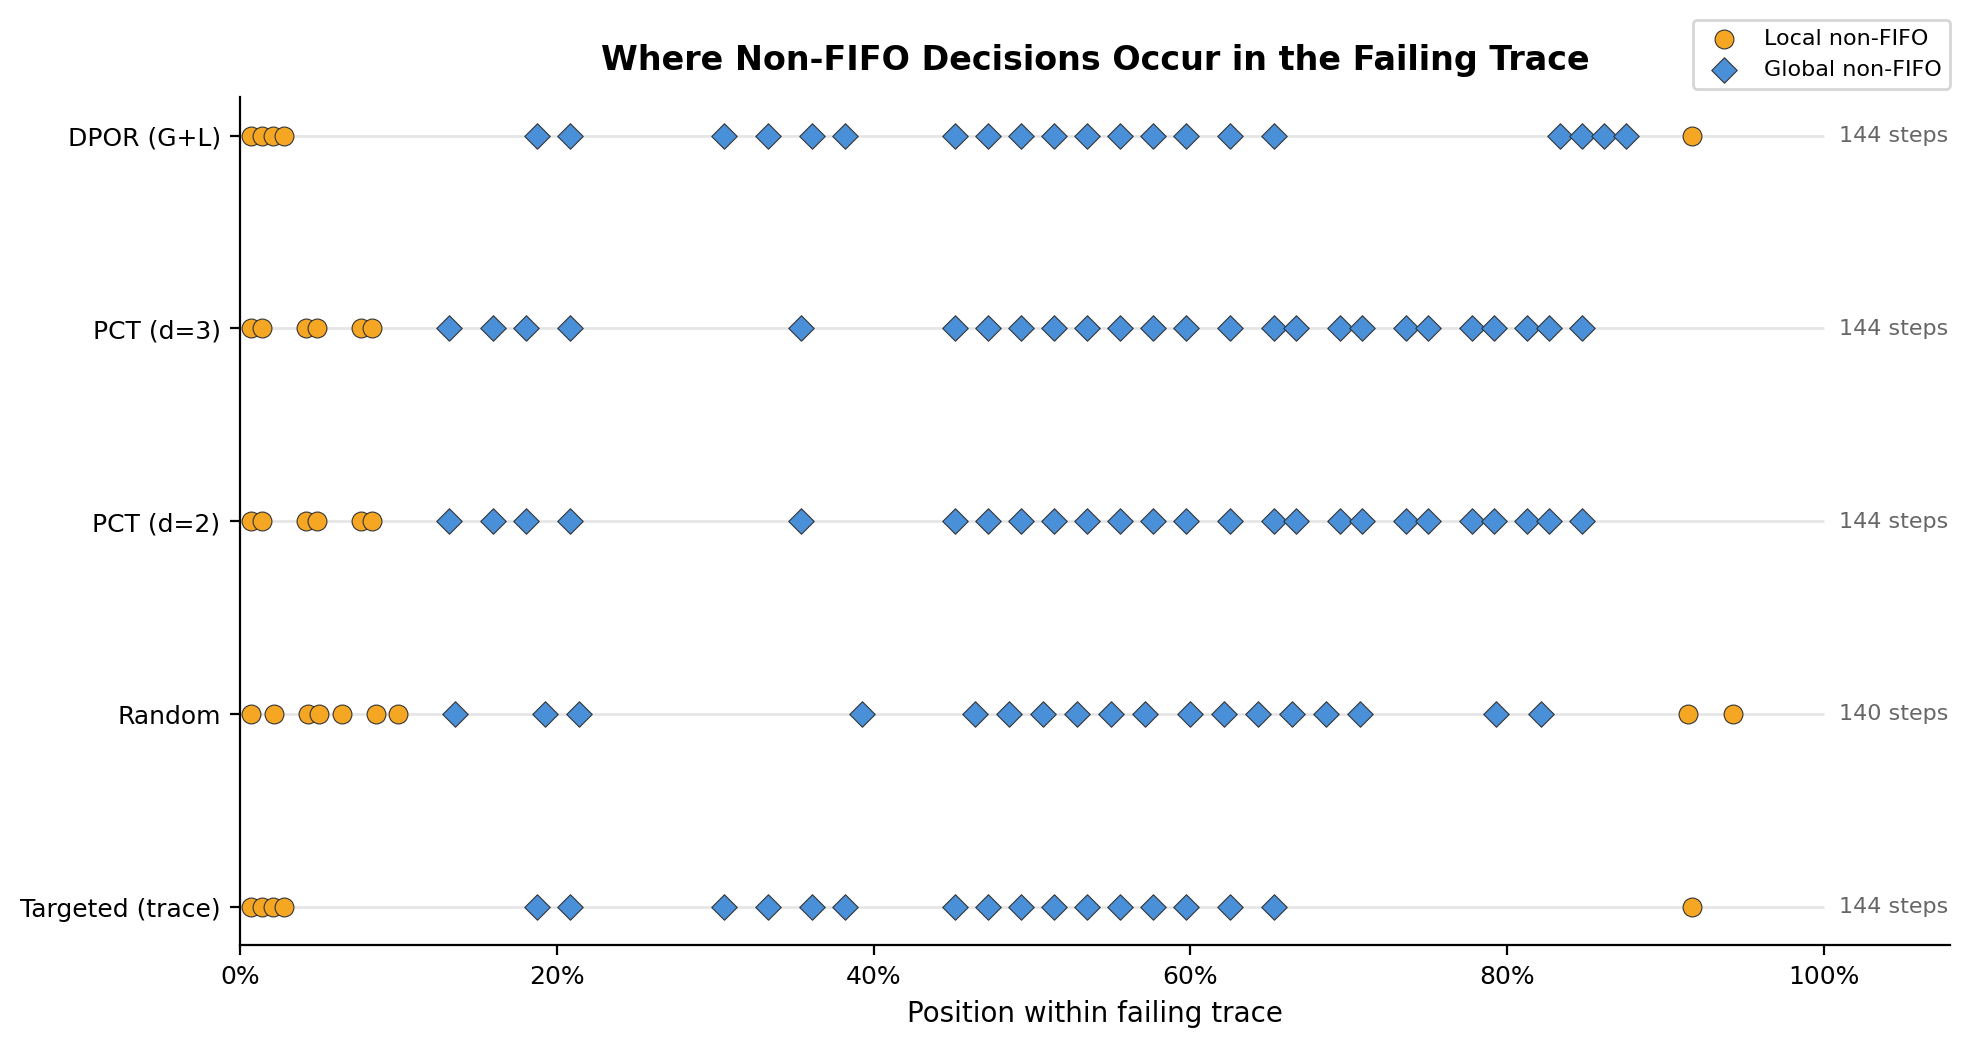
\includegraphics[width=0.85\linewidth]{../../bugs/quorum-read-repair/benchmarking/figures/nonfifo_position_profile.png}
  \caption{Position of non-FIFO decisions within the bug-finding trace, as a fraction of total trace length. Local (orange) decisions cluster in the first 10\% of the trace for all algorithms. Global (blue) decisions are spread across the middle of the trace. DPOR's local decisions are denser at the front, reflecting its systematic exploration of the early goroutine scheduling space.}
  \label{fig:qrr-pos}
\end{figure}

Figure~\ref{fig:qrr-pos} shows where the non-FIFO decisions fall within the trace. Local non-FIFO decisions appear in the first 10\% of the trace for all algorithms --- this is where R1's internal pipeline is most active, immediately after messages are delivered. The critical goroutine sequence (router $\to$ router $\to$ repairLoop $\to$ applyLoop) must happen early, before the pipeline drains naturally. Global non-FIFO decisions are distributed across the middle of the trace, reflecting the message reordering needed to route Reader's quorum read through the stale R1 path and then race the late Put against the Repair. DPOR's local decisions are notably denser at the front than PCT's, consistent with its systematic enumeration of early local alternatives rather than a single lucky assignment.

\begin{figure}[h]
  \centering
  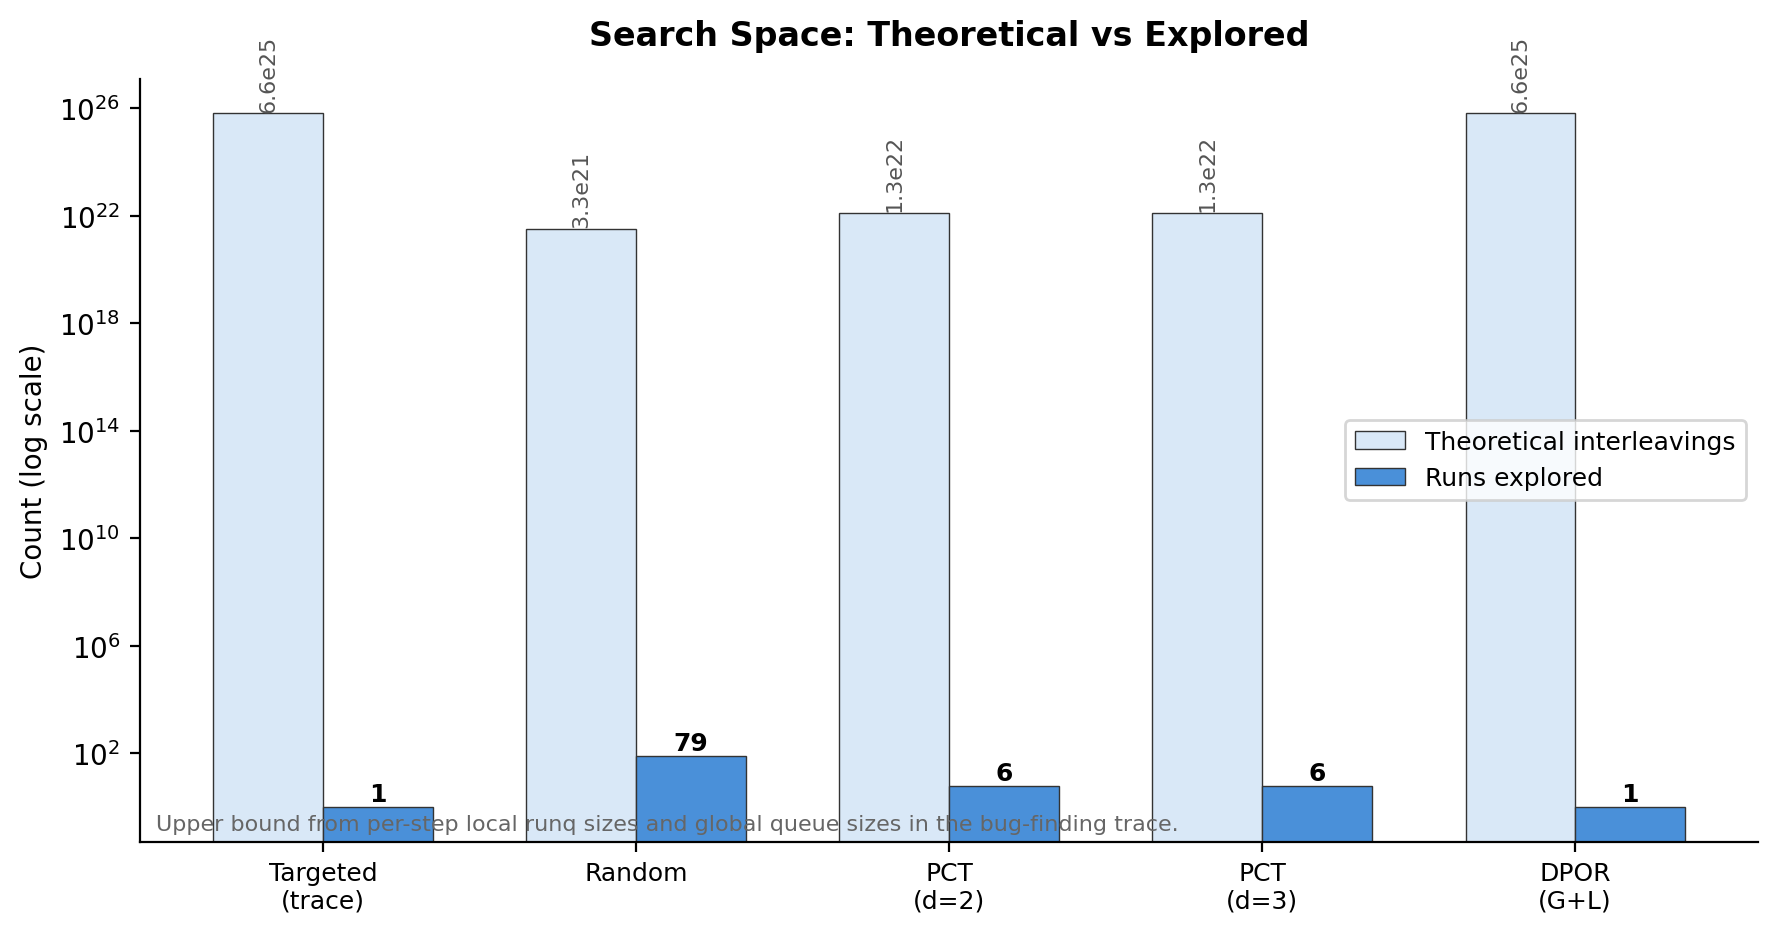
\includegraphics[width=0.85\linewidth]{../../bugs/quorum-read-repair/benchmarking/figures/search_space_vs_explored.png}
  \caption{Theoretical search space size versus number of runs explored to find the bug. DPOR's pruned space ($2.2 \times 10^{18}$) is four orders of magnitude smaller than PCT's unpruned space ($1.3 \times 10^{22}$). Despite the smaller space, DPOR explores 11 traces to PCT's 6 --- the pruning changes the geometry, not just the size.}
  \label{fig:qrr-space}
\end{figure}

Figure~\ref{fig:qrr-space} quantifies the payoff from DPOR's partial order reduction. DPOR's effective search space is $2.2 \times 10^{18}$, four orders of magnitude smaller than the unpruned space of $1.3 \times 10^{22}$ that PCT and Random must navigate. The reduction comes from identifying commutative interleavings --- pairs of message deliveries or goroutine scheduling choices that produce equivalent outcomes regardless of order --- and collapsing them into a single representative trace. DPOR explores only one member of each equivalence class, skipping the rest by construction. Despite operating in a smaller space, DPOR still needs 11 runs to PCT's 6: the pruning changes the geometry of the space, not just its size, and the bug-triggering trace happens to appear at position 11 in DPOR's deterministic traversal of the pruned space.

\subsection{Discussion}

The two distributed bugs together demonstrate a coverage complementarity across strategies:

\textbf{CHESS} provides complete systematic coverage within its bound and is the right choice when bugs are expected to require few non-FIFO decisions. It found 11/14 GoBench bugs and the ra-gate bug reliably, but is structurally blind to quorum-read-repair.

\textbf{DPOR} prunes independent interleavings and arrives at deep bugs via shorter, more targeted paths. It is deterministic (same result every seed) and found quorum-read-repair in a fixed 11-run path, but does not provide the exhaustiveness guarantee that CHESS offers.

\textbf{PCT} is the best probabilistic option when the per-run probability of hitting the bug is non-negligible. It found ra-gate in a single run and quorum-read-repair in under 7 runs on average --- faster than both CHESS and DPOR in terms of raw runs-to-bug. The tradeoff is that it offers no completeness guarantee and requires tuning the depth parameter $d$.

\textbf{Local scheduling matters.} The CHESS global-only failure on ra-gate (6/20 attempts) shows that message reordering alone is not sufficient to test all distributed concurrency bugs. A framework that only varies message delivery order --- as most distributed testing tools do --- would miss any bug that requires a specific goroutine interleaving within a node.

\textbf{Context bound limitations.} Quorum-read-repair demonstrates a hard boundary for CHESS: if the bug requires more than $k$ non-FIFO steps, the algorithm cannot find it no matter how long it runs. Practical distributed systems with deep pipelines or multi-stage commit protocols may have bugs of this kind, making bound-free algorithms like DPOR or PCT necessary complements to CHESS.

\appendix

\section{ra-gate: Full Bug Description}
\label{app:ra-gate}

\textit{[Placeholder: full long-form description from Google Docs goes here. Include: Ricart-Agrawala protocol background, the close(gate) pattern, the three-goroutine structure (Handler, App, DeferredFlusher), the exact conditions that trigger the violation, and a trace walkthrough of the bug-finding run.]}

\section{Quorum Read-Repair: Full Bug Description}
\label{app:quorum-read-repair}

\textit{[Placeholder: full long-form description from Google Docs goes here. Include: Dynamo-style replication model, vector clock merge semantics, the router/applyLoop pipeline, the pendingApply race window, the read-repair trigger, and a trace walkthrough showing how the lost sibling manifests.]}


\end{document}
